\section{Exercises}

\begin{enumerate}[leftmargin=*]
\item Determine whether the statement is {\bf True} or {\bf False}.
\begin{enumerate}
\item Let $ \boldsymbol{v}_1 , \boldsymbol{v}_2 \in \mathbb{R}^2 $ be linearly independent vectors. Let $ \lambda_1 , \lambda_2 $ be real numbers. Then there exists a unique 2 by 2 matrix $ A $ with eigenvalues $ \lambda_1 , \lambda_2 $ and corresponding eigenvectors $ \boldsymbol{v}_1 , \boldsymbol{v}_2 $.
\item The singular value decomposition $A = P\Sigma Q^T$ is unique.
\item The inverse iteration algorithm (without normalization) computes a recursive sequence $ A \boldsymbol{x}_{k+1} = \boldsymbol{x}_k $ where $ \boldsymbol{x}_k $ converges to:
\begin{enumerate}
\item the largest (in absolute value $ | \lambda | $) eigenvalue of $ A $
\item an eigenvector corresponding to the largest (in absolute value $ | \lambda | $) eigenvalue of $ A $
\item the smallest (in absolute value $ | \lambda | $) eigenvalue of $ A $
\item an eigenvector corresponding to the smallest (in absolute value $ | \lambda | $) eigenvalue of $ A $
\end{enumerate}
\item In the power iteration algorithm, we divide by $ \| A \boldsymbol{x}_k \|_{\infty} $ in each step to:
\begin{enumerate}
\item make the algorithm run faster
\item prevent the entries of the vectors $ \boldsymbol{x}_k $ from becoming too large/small
\item produce a more accurate result
\end{enumerate}
\item Let $ \lambda $ be a (nonzero) eigenvalue of an invertible matrix $ A $.
\begin{enumerate}
\item $ \lambda^{-1} $ is an eigenvalue of $ A^{-1} $
\item $ \lambda $ is an eigenvalue of $ A^T $
\item $ \lambda^2 $ is an eigenvalue of $ AA^T $
\item $ \lambda $ is an eigenvalue of $ PAP^{-1} $ for any invertible matrix $ P $
\item $ \lambda \not= 0 $
\end{enumerate}
\item Let $ \boldsymbol{u} \in \mathbb{R}^n $ be a nonzero vector and let $ H = I - \frac{2}{\| \boldsymbol{u} \|^2} \boldsymbol{u} \boldsymbol{u}^T $ be the corresponding elementary reflector. Then $\lambda = -1$ is an eigenvalue of $H$ with multiplicity 1.
\item Let $ U \subset \mathbb{R}^n $ be a subspace with $ \mathrm{dim}(U) = m $ such that $ 0 < m < n$, and let $ P $ be the orthogonal projection matrix onto $ U $. Then $ \lambda = 0 $ is an eigenvalue for $ P $ with multiplicity $ m $.
\item Suppose $A$ and $B$ are symmetric $n \times n$ matrices. Then the eigenvectors of $AB$ corresponding to distinct eigenvalues are orthogonal.
\item Let $ A $ be any $ m \times n $ matrix. If $ \lambda $ is an eigenvalue of $ AA^T $ then $ \lambda $ is a real number and $ \lambda \geq 0 $.
\item Let $ A $ be any $ m \times n $ matrix. If $ \boldsymbol{v}_1 , \boldsymbol{v}_2 $ are eigenvectors of $ AA^T $ for distinct eigenvalues then $ \boldsymbol{v}_1 \cdot \boldsymbol{v}_1 = 0 $.
\item Let $ \boldsymbol{u} \in \mathbb{R}^n $ and let $ H = I - \frac{2}{\| \boldsymbol{u} \|^2} \boldsymbol{u} \boldsymbol{u}^T $ be the corresponding elementary reflector. The characteristic polynomial of $ H $ is $ (x-1)^{n-1}(x+1)$.
\item Let $ P $ be an orthogonal projection matrix. All the eigenvalues of $ P $ are either 1 or 0.
\item Let $ \lambda $ be an eigenvalue of an invertible matrix $ A $. Identify all True statements:
\begin{enumerate}
\item $ \lambda^{-1} $ is an eigenvalue of $ A^{-1} $
\item $ \lambda $ is an eigenvalue of $ A^T $
\item $ \lambda^2 $ is an eigenvalue of $ AA^T $
\item $ \lambda $ is an eigenvalue of $ PAP^{-1} $ for any invertible matrix $ P $
\item $ \lambda \not= 0 $
\end{enumerate}
\end{enumerate}
\item Let $ A $ be a $ 2 \times 2 $ matrix with eigenvalues $ \lambda_1 = 1 $ and $ \lambda_2 = 1/2 $ and corresponding eigenvectors
\[ \boldsymbol{v}_1 = \begin{bmatrix} 1 \\ 2 \end{bmatrix} \hspace{10mm} \boldsymbol{v}_2 = \begin{bmatrix} -1 \\ 1 \end{bmatrix} \]
If we choose $ \boldsymbol{x}_0 = \begin{bmatrix} 1 \\ 5 \end{bmatrix} $ then the sequence $ \boldsymbol{x}_{k+1} = A \boldsymbol{x}_k $ converges to what?
\item Find the singular value decomposition of $\displaystyle A = \left[ \begin{array}{rrr} 1 & \ \, 2 & -1 \\ 2 & 1 & 4 \end{array} \right]$.
\item Suppose $ A $ is a symmetric $ 3 \times 3 $ matrix with distinct eigenvalues $ \lambda_1 , \lambda_2 , \lambda_3 $ and eigenvectors
\[ \boldsymbol{v}_1 = \begin{bmatrix} 1 \\ 1 \\ 1 \end{bmatrix} \hspace{10mm} \boldsymbol{v}_2 = \begin{bmatrix} 1 \\ 0 \\ -1 \end{bmatrix} \]
Determine eigenvector $ \boldsymbol{v}_3 $ for eigenvalue $ \lambda_3 $.
\item Find the singular value decomposition of $ \displaystyle A = \left[ \begin{array}{rrr} 1 & 1 & 1 \\ -1 & 2 & -1 \\ 1 & 0 & -1 \end{array} \right] $.
\item Determine whether the statement is {\bf True} or {\bf False}. (Assume all data matrices are normalized.)
\begin{enumerate}
\item Let $X$ be a $n \times p$ data matrix and let $\bs{x}_i , \bs{x}_j \in \mathbb{R}^p$ be two different rows of $X$ such that $\| \bs{x}_i \| < \| \bs{x}_j \|$. If $\bs{w}_1$ is the first weight vector of $X$, then $| \bs{x}_i \cdot \bs{w}_1 | < | \bs{x}_j \cdot \bs{w}_1 |$.
\item Let $X$ be a $n \times p$ data matrix and let $\bs{x}_i , \bs{x}_j \in \mathbb{R}^p$ be two different rows of $X$ such that $\bs{x}_i \cdot \bs{x}_j = 0$. If $\bs{w}_1$ is the first weight vector of $X$ and $\bs{x}_i \cdot \bs{w}_1 = 0$ then $\bs{x}_j \cdot \bs{w}_1 = 0$.
\item Let $X$ be a $n \times 2$ data matrix and let $Y$ be the matrix with the same columns as $X$ but switched. (In other words, the first column of $Y$ is the same as the second column of $X$, and the second column of $Y$ is the first column of $X$.) If $X$ and $Y$ represent the same set of data points, then all the singular values of $X$ equal.
\item Let $X$ be a $n \times 2$ data matrix and let $Y$ be the matrix with the same columns as $X$ but switched. (In other words, the first column of $Y$ is the same as the second column of $X$, and the second column of $Y$ is the first column of $X$.) If $X$ and $Y$ represent the same set of data points, then $\bs{w}_1 = \begin{bmatrix} 1/\sqrt{2} & 1/\sqrt{2} \end{bmatrix}^T$.
\item It is necessary to compute all the eigenvectors of the Google matrix to find the PageRank vector of a directed graph.
\end{enumerate}
\item Find the weight vectors for the data matrix $X$ representing the points:
\begin{center}
\includegraphics[width=3in]{03_04_ex01.png}
\end{center}
\item Suppose $X$ is a $100 \times 4$ data matrix such that
$$
X^T X = \begin{bmatrix} 2 & 0 & 0 & 0 \\ 0 & 1.5 & 0 & 0 \\ 0 & 0 & 2 & 1 \\ 0 & 0 & 1 & 2 \end{bmatrix}
$$
Find all the weight vectors of $X$.
\item Suppose we want to solve a system $A \bs{x} = \bs{b}$. A small change $\Delta \bs{b}$ produces a change in the solution
$$
A(\bs{x} + \Delta \bs{x}) = \bs{b} + \Delta \bs{b}
$$
Describe the unit vector $\Delta \bs{b}$ that will produce the largest change $\| \Delta \bs{x} \|$.
\item Find the rank 2 pseudo inverse
$$
A_2^+ = \frac{1}{\sigma_1} \bs{q}_1 \bs{p}_1^T + \frac{1}{\sigma_2} \bs{q}_2 \bs{p}_2^T
$$
of the matrix
$$
A = \left[ \begin{array}{rrr} 1 & 1 & 1 \\ 1 & 0 & -2 \\ 1 & -1 & 1 \end{array} \right]
$$
(Note: the columns of $A$ are orthogonal.)
\item Let $A$ be a $m \times n$ matrix with singular value decomposition $A = P \Sigma Q^T$. Let $k < \min\{m,n\}$ and let
$$
A_k = \sum_{i=1}^k \sigma_i \bs{p}_i \bs{q}_i^T
$$
Describe the singular value decomposition of $A - A_k$.
%\item Consider a Toeplitz matrix of the form
%$$
%A = 
%\begin{bmatrix}
%a & b & & & \\
%c & a & b & & \\
% &  & \ddots & & \\
% & & c & a & b \\
% & & & c & a
%\end{bmatrix}
%$$
%and an image matrix $X$
%\begin{enumerate}
%\item If $c > a > b > 0$, would the blurred image $AX$ look more blurred upward or downward?
%\item If $c > a > b > 0$, would the blurred image $XA^T$ look more blurred to the right or left?
%\end{enumerate}
\item Consider the same directed graph as in the example in the section on PageRank:
\begin{center}
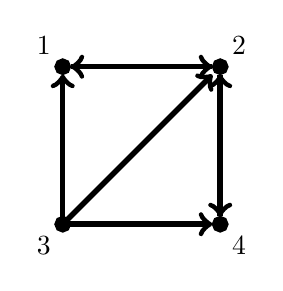
\begin{tikzpicture}[scale=2.0,line width=2pt]
\filldraw (0,0) circle (1pt); \filldraw (0,1) circle (1pt);
\filldraw (1,1) circle (1pt); \filldraw (1,0) circle (1pt);
\draw (0,1) node[anchor=south east] {1};
\draw (1,1) node[anchor=south west] {2};
\draw (1,0) node[anchor=north west] {4};
\draw (0,0) node[anchor=north east] {3};
\draw [->] (0,0) to (0,0.95);
\draw [->] (0,0) to (0.95,0);
\draw [->] (0,0) to (0.95,0.95);
\draw [->] (1,0.95) to (1,0.05);
\draw [->] (1,0.05) to (1,0.95);
\draw [->] (0.05,1) to (0.95,1);
\draw [->] (0.95,1) to (0.05,1);
\end{tikzpicture}
\end{center}
As $\alpha \to 1$, describe what happens to the PageRank $x_3$ of vertex 3.
\item Let $G$ be the complete directed graph with $N$ vertices. In other words, there is an edge from each vertex to every other vertex in $G$ (excluding edges from a vertex to itself). Describe the Google matrix and the PageRank vector for the complete directed graph.
\item Find the Google matrix $\alpha P + (1 - \alpha) \bs{v} \bs{e}^T$ for the directed graph
\begin{center}
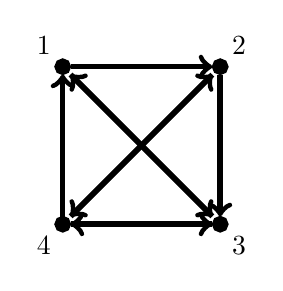
\begin{tikzpicture}[scale=2.0,line width=2pt]
\filldraw (0,0) circle (1pt); \filldraw (0,1) circle (1pt);
\filldraw (1,1) circle (1pt); \filldraw (1,0) circle (1pt);
\draw (0,1) node[anchor=south east] {1};
\draw (1,1) node[anchor=south west] {2};
\draw (1,0) node[anchor=north west] {3};
\draw (0,0) node[anchor=north east] {4};
\draw [->] (0,0) to (0,0.95);
\draw [->] (0.05,0) to (0.95,0);
\draw [->] (0.95,0) to (0.05,0);
\draw [->] (0.05,0.05) to (0.95,0.95);
\draw [->] (0.95,0.95) to (0.05,0.05);
\draw [->] (0.05,0.95) to (0.95,0.05);
\draw [->] (0.95,0.05) to (0.05,0.95);
\draw [->] (1,0.95) to (1,0.05);
\draw [->] (0.05,1) to (0.95,1);

%\draw [->] (0.05,1.05) to[out=45,in=135] (0.95,1.07);
%\draw [->] (0.05,1) to[out=0,in=90] (1,0.1);
%\draw [->] (0.95,0) to[out=180,in=-90] (0,0.9);
%\draw [->] (0.05,0.05) to[out=45,in=135] (0.9,0.05);
%\draw [->] (0.95,-0.05) to[in=-45,out=225] (0.07,-0.07);
%\draw [->] (-0.05,0.05) to[out=135,in=225] (-0.1,0.95);
%\draw [->] (1.05,0.95) to[out=-45,in=45] (1.1,0.05);
%\draw [->] (0,0.05) to[out=90,in=180] (0.9,1);
%\draw [->] (1,0.95) to[out=-90,in=0] (0.1,0);
\end{tikzpicture}
\end{center}
using teleportation parameter $\alpha=0.5$ and uniform distribution vector $\bs{v}$. Let $\bs{x}_0 = \begin{bmatrix} 1 & 0 & 0 & 0 \end{bmatrix}^T$ and use Python to compute 50 iterations of the power method to approximate the PageRank vector.
\item Find the Google matrix $\alpha P + (1 - \alpha) \bs{v} \bs{e}^T$ for the directed graph in the previous exercise using teleportation parameter $\alpha=0.8$ and distribution vector $\bs{v} =  \begin{bmatrix} 0 & 1/2 & 1/2 & 0 \end{bmatrix}^T$. Let $\bs{x}_0 = \begin{bmatrix} 1 & 0 & 0 & 0 \end{bmatrix}^T$ and use Python to compute 50 iterations of the power method to approximate the PageRank vector.
\end{enumerate}